\section{Introduction}
In modern embedded and high performance computing systems, there is increasing interest in \textit{spatial processors}. These processing architectures consisting of physically distributed Processing Elements (PEs), and are more energy efficient than traditional general purpose processors and reconfigurable hardware accelerators.~\cite{parashar2014efficient,prabhakar2017plasticine,budiu2004spatial,streamproc2019,cerqueira2020catena,7284058,8686088}. %thus matching current application demands.
%ADD CITATION ((2013). The End of Dennard Scaling. Accessed: Feb. 2013. [Online].
%Available: https://cartesianproduct.wordpress.com/2013/04/15/the-endof-dennard-scaling/
%[3] H. Esmaeilzadeh, E. Blem, R. S. Amant, K. Sankaralingam, and
%D. Burger, “Dark silicon and the end of multicore scaling,” in Proc.
%38th Annu. Int. Symp. Comput. Archit. (ISCA), Jun. 2011, pp. 365–376.}
Despite the growing interest, we are still far from having the right  solutions and automated tools for designing efficient, high-performance spatial processors. An important drawback of existing design solutions is their inability to take the memory system into account, despite compelling evidence that the memory system (both on-chip and off-chip) has become a dominant factor affecting the overall performance, power consumption, and silicon area usage~\cite{williams2009roofline,dayarathna2015data,oh2009analytical}.
In this work we argue that, given that the memory system and the processing elements in a spatial processor architecture are so tightly \textit{interdependent}, they must be \textit{co-designed} to efficiently use the available resources. A memory-aware design produces spatial architectures having bandwidth close to the bandwidth of the memory system, effectively reducing the instantiation of unrequired resources. Co-designing becomes especially important when considering the use of emerging memory technologies, such as MRAM, eDRAM, PCM, or RRAM~\cite{mem2016} in spatial processors: they have higher integration density and lower power than SRAM, but also come with additional "quirks" (e.g., MRAM features different read and write latencies).

%
%BibTeX | EndNote | ACM Ref
%@inproceedings{Hameed:2010:USI:1815961.1815968,
% author = {Hameed, Rehan and Qadeer, Wajahat and Wachs, Megan and Azizi, Omid and Solomatnikov, Alex and Lee, Benjamin C. and Richardson, Stephen and Kozyrakis, Christos and Horowitz, Mark},
% title = {Understanding Sources of Inefficiency in General-purpose Chips},
% booktitle = {Proceedings of the 37th Annual International Symposium on Computer Architecture},
% series = {ISCA '10},
% year = {2010},
% isbn = {978-1-4503-0053-7},
% location = {Saint-Malo, France},
% pages = {37--47},
% numpages = {11},
% url = {http://doi.acm.org/10.1145/1815961.1815968},
% doi = {10.1145/1815961.1815968},
% acmid = {1815968},
% publisher = {ACM},
% address = {New York, NY, USA},
% keywords = {ASIC, chip multiprocessor, customization, energy efficiency, h.264, high performance, tensilica},
%}

There are CAD tools~\cite{synopsystool,tensilica,codasiptool} that reduce the increasing design complexity of typical application-specific processors. However, selecting an optimal spatial processor architecture, taking into account the various trade-offs in latency, power consumption, and area usage still requires extensive design-space exploration (DSE) and cannot be performed using the existing CAD tools.
%In addition, state-of-the-art design flows for application-specific processor DSE focus on processing elements optimization~\cite{Meloni2012,EusseSAMOS2014,Jozwiak2013,Karuri2009}, and do not include the memory system, as illustrated in Figure~\ref{fig:intro}. Instead, co-optimization of the processor and the memory system (including emerging memories) is typically done through the optimization of cache replacement policies~\cite{4798259,7092595,6271803,Mittal13f}.
In addition, state-of-the-art design flows for application-specific processor DSE focus on processing elements optimization~\cite{Meloni2012,EusseSAMOS2014,Jozwiak2013}, and do not include the memory system, as illustrated in Figure~\ref{fig:intro}. Instead, co-optimization of the processor and the memory system (including emerging memories) is typically done through the optimization of cache replacement policies~\cite{4798259,7092595,6271803}.
%Papers to cite for CDFG generation and Application Specific High LSynthesis~\cite{Coussy:2008:HSA:1457713,Kato2008}.
%On the other hand, emerging spatial architectures~\cite{7284058,8686088}, which distribute the program memory and processing elements to achieve maximum performance use rigid interconnect topologies to allow flexible communication between processing elements leading to larger area and power utilization.

\begin{figure}[ht]
    \centering
    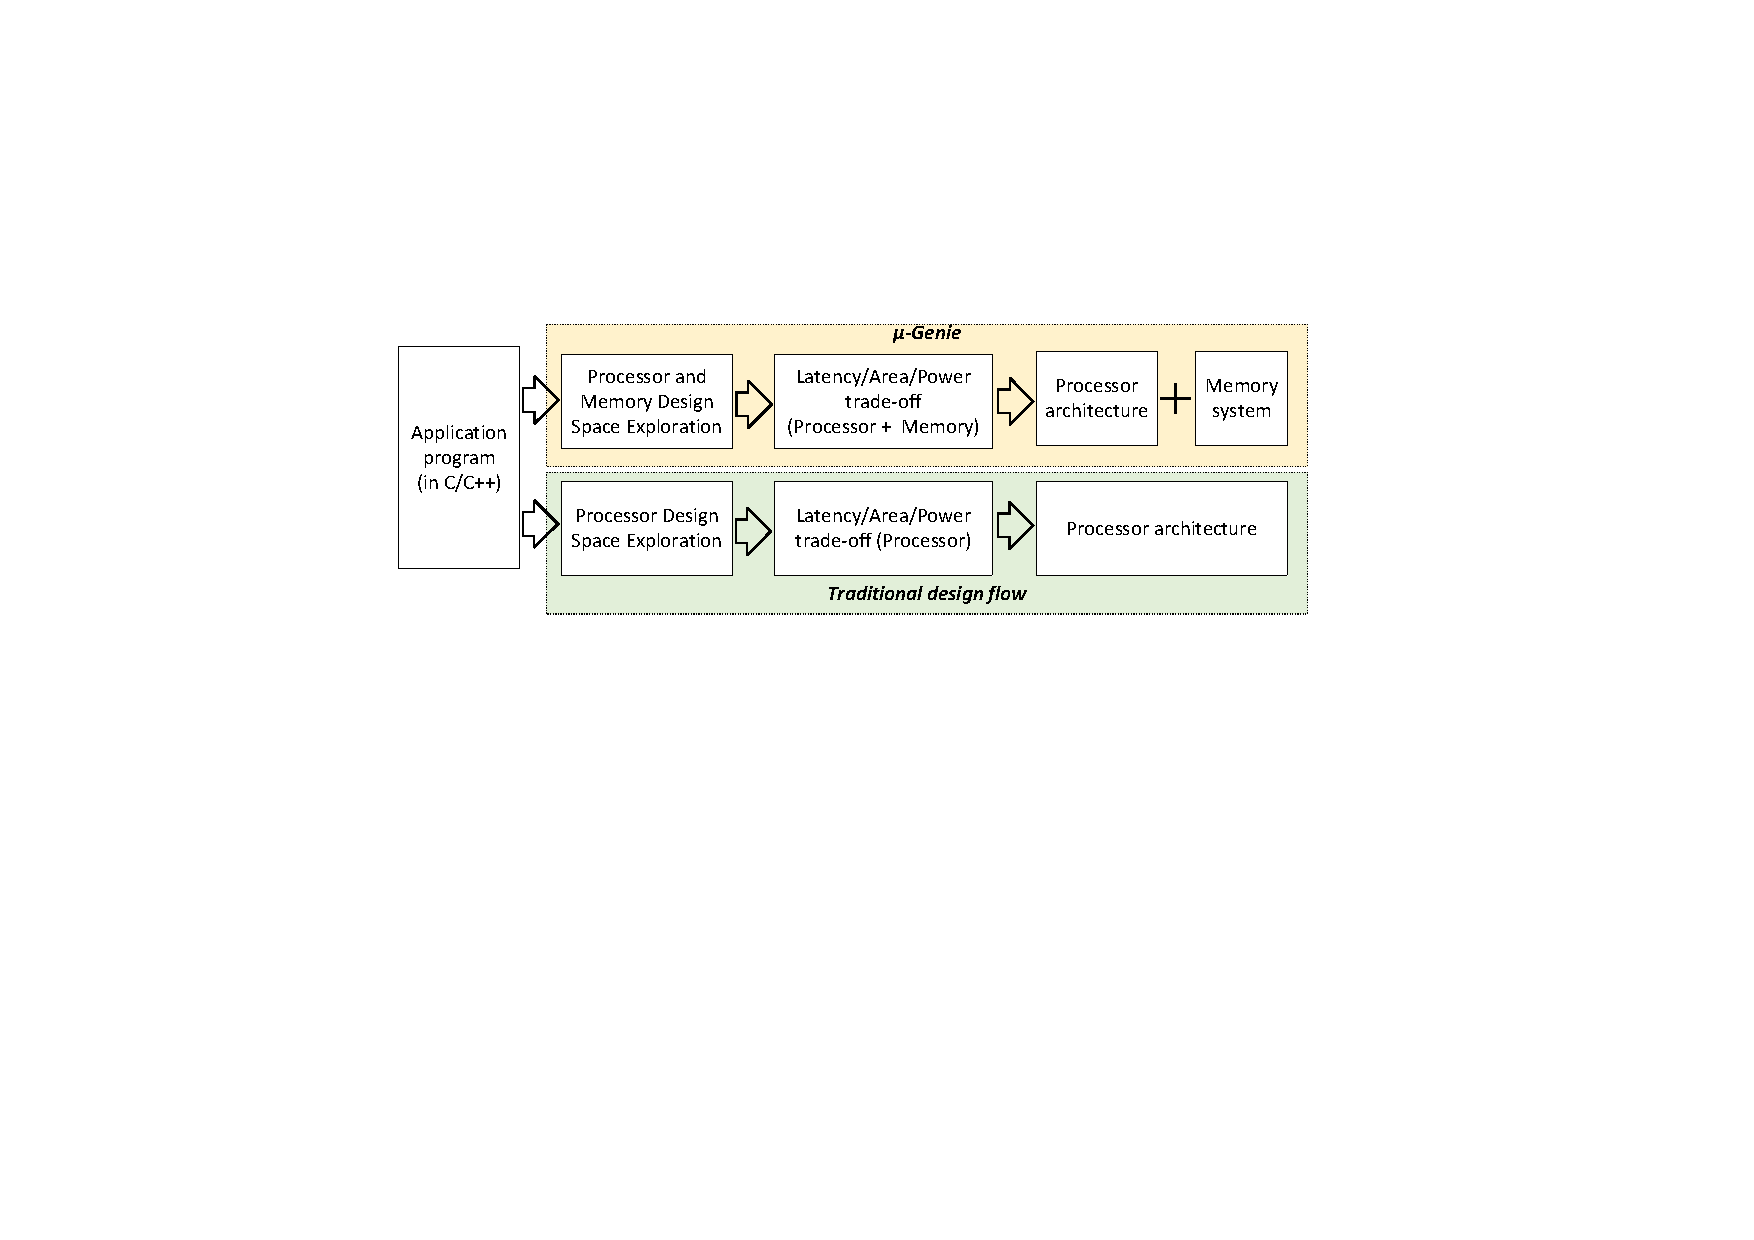
\includegraphics[clip, trim=6cm 10.5cm 6.4cm 5.2cm, width=1.0\linewidth]{images/intro_figure.pdf} %[left down right up ]
    \caption{\small Difference between state-of-the-art design flow typically used for traditional application-specific processors and the proposed \frameworkname~design flow for spatial processors.}
    \label{fig:intro}
\end{figure}

This paper presents as main contribution \frameworkname~(Section~\ref{sec:framework}), an automated framework for \textit{memory-aware spatial processor design-space exploration}. The framework presented in this work allows the user to \textbf{customize} the different building blocks to be used in the co-design of the spatial processor and memory system, \textbf{explore} different architectures automatically generated for a given application, and \textbf{estimate} area, power and latency of each one of the architectures.
We highlight as key novel contributions:

1. Unprecedented configuration options: memory levels technologies (novel among similar tools), clock frequency (per memory level, also novel), different read/write latencies, and data-widths.

2. A configurable PE architecture template (Section~\ref{sec:arch_template}) that allows fast prototyping of spatial processor hardware.

3. The Modified Interval Partitioning (MIP) algorithm (Section~\ref{ssec:modified_interval_partitioning}), that enables the memory-aware co-Design Space Exploration (Section~\ref{ssec:dse}).

To demonstrate the capabilities of \frameworkname, we cover three case-studies, showing how a spatial processor can be designed for two different applications and many configurations, including those using MRAM or SRAM for the memory system, can be generated, analyzed, and compared (Section~\ref{sec:case_studies}).



 %Ana: if you keep this format, without the contributions specifically listed, this final paragraph (below) is not well-positioned. You might want ti add this at the beginning of "In this work..." paragraph - I added it there for you to see what I mean. This summary is only needed here if you go for the bullet-point-like contributions.
 %\frameworkname~enables design space exploration for application-specific custom-processors beyond the current state-of-the-art solutions, even enabling a first comparison between different memory technologies, like MRAM and SRAM.

%In this work we present \frameworkname, a framework that allows to compare design choices and perform automatic system level design and implementation. We propose a novel memory-driven approach for application-specific hardware design starting from two observations. First, the memory system and the processing system are \textit{interdependent} and therefore they should be \textit{co-designed}. Second, the \textit{data dependencies} of the fixed application impose constaints on the design of both memory and processing systems. Hence, our approach starts from the analysis of an input application and codesigns memory and custom processor, shown in Figure~\ref{fig:intro}.
